\section{Mediciones}\label{sec:mediciones}

\subsection{Primera medición}\label{subsec:medicion1}
\subsubsection{Procesamiento y generación de datos de entrada:} 
Se realizaron mediciones en base a crear arreglos para $x$ y $f$ de diferentes largos, yendo de 100 en 100 minutos, para los cuales, en cada caso, los elementos de $x$ fueron generados por los valores pseudoaleatorios del lenguaje (el módulo \texttt{random}) y los elemenos de $f$, generados de forma creciente a pasos, igualmente, de valores pseudoaleatorios. 

En esta ocación no fue necesario estabilizar los resultados, se muestran de forma clara en el gráfico.

\begin{figure}[H]
    \centering
    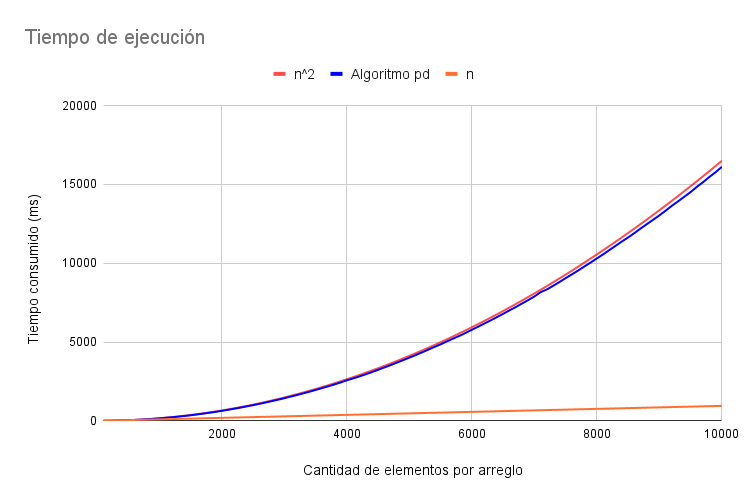
\includegraphics[width=1\textwidth]{img/tiempos_10k_100.png}
    \caption{Medición 1}
\end{figure}

\subsubsection{Análisis de los resultados:}
Con estos resultados es preciso el poder afirmar que el algoritmo PD propuesto, si bien está optimizado para casos particulares, efectivamente tiene una tendencia \textbf{cuadrática} en función del tamaño de los datos de entrada, exactamente como es esperado.
\newpage

\subsection{Segunda medición: Caso particular $x_i$ y $f_i$ constantes}

\subsubsection{Procesamiento y generación de datos de entrada:} 
En este caso se realizaron mediciones en base a crear arreglos de diferentes largos con elementos de valores constantes $C$ y $K$ para $x$ y $f$ respectivamente, yendo de  100 en 100 minutos, cumpliendo $C < K$.

Para obtener un gráfico más legible, los resultados fueron estabilizados usando el promedio de tiempo de 3 por cada prueba.

\begin{figure}[H]
    \centering
    \includegraphics[width=1\textwidth]{img/tiempos_10k_100_xi<f0_constantes.png}
    \caption{Medición 2}
\end{figure}

\subsubsection{Análisis de los resultados:}
Haciendo mediciones con $C < K$ entramos al caso particular $x_i < f_0\forall i $, donde no solo nos encontramos ante una mejora muy significativa en los tiempos del algoritmo, sino además una tendencia \textbf{lineal}. Estos resultados si bien son los esperados debido a la optimización aplicada a nuestro algoritmo, al ser $K$ constante para todo valor de $f$, nos encontramos en un entorno alejado de la realidad, pues los valores de $f$ a recibir serían estrictamente crecientes. 

\newpage

\subsection{Tercera medición: Caso particular $x_i$ y $f_i$ variables}

\subsubsection{Procesamiento y generación de datos de entrada:} 
En este caso, tal como en la \textit{Medición 1}(véase \ref{subsec:medicion1}), se realizaron mediciones en base a crear arreglos para $x$ y $f$ de diferentes largos, yendo de 100 en 100 minutos, con valores pseudoaleatorios para $x$ y pasos pseudoaleatorios para $f$, pero asegurando $x_i < f_0 \forall i $.

Para obtener un gráfico más legible, los resultados fueron estabilizados usando el promedio de tiempo de 3 por cada prueba.

\begin{figure}[H]
    \centering
    \includegraphics[width=1\textwidth]{img/tiempos_10k_100_xi<f0_no_constantes.png}
    \caption{Medición 3}
\end{figure}

\subsubsection{Análisis de los resultados:}
Con estos resultados podemos afirmar que haciendo mediciones con $x_i < f_0 \forall i $ con valores para x y f variables, la optimización efectivamente conlleva a una tendencia \textbf{lineal} y a una significativa mejoría en los tiempos de ejecución de nuestro algoritmo. Cabe aclarar que esta medición refleja el caso en el que nuestra optimización abarca la mayor cantidad de minutos que puede abarcar ($n$) para todas las batallas examinadas pero no es el único caso en el que este se aplique, los minutos pueden variar.
\newpage
